\subsection{Root Cause Analysis}


\subsubsection*{Problem}


Der Fehler (fault) A wird zum Error (error) A und führt zum System Fehler (failure) A. Dieser führt zu Fehler B. Fehler B wird zum Error und führt zum System Fehler B. Dies kann unter Umständen immer so weiter gehen, dabei werden die einzelnen Fehler vom System geloggt. Das System hat inzwischen den Fehler behoben und arbeitet normal weiter. Jetzt ist es an der Zeit den Fehler zu analysieren und zu beheben, welcher den Error verursacht hat.

\begin{figure}[H]
	\centering
	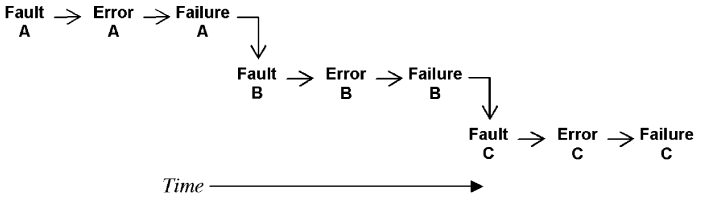
\includegraphics[width=\textwidth]{content/faulttolerance/images/failureSequence.PNG}
	\caption{failureSequence}
\end{figure}


Wie bereits angedeutet, kann der erkannte Error die Ursache für weitere Failure sein. Und umgekehrt, kann ein Error auch mehrere Faults als Vorgänger haben.

\subsubsection*{Lösung}


\begin{figure}[H]
	\centering
	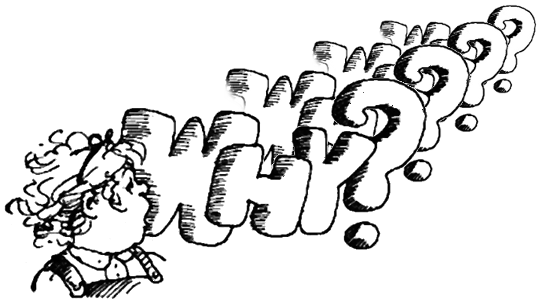
\includegraphics[width=\textwidth]{content/faulttolerance/images/why.png}
	\caption{why}
\end{figure}


Um einen Error zu beheben muss das Problem bei der Wurzel gelöst werden, also beim ursprünglichen Verursacher des Errors, auch root cause genannt. Dieser Fault muss als erstes korrigiert werden. Danach werden alle weiteren Faults nach und nach bis zum verursachenden Fault korrigiert. Um den sogenannten root cause zu finden, kann die 5 Warum-Fragetechnik verwendet werden.

\begin{itemize}
	\item Why was the data record lost?
	\begin{itemize}
		\item Because the transaction failed in the middle.
	\end{itemize}
	\item Why did the transaction fail in the middle?
	\begin{itemize}
		\item Because it ran out of memory.
	\end{itemize}
	\item Why did it run out of memory?
	\begin{itemize}
		\item Because there was no more memory available for allocation.
	\end{itemize}
	\item Why was there no more memory available for allocation?
	\begin{itemize}
		\item Because the memory was inaccessible.
	\end{itemize}
	\item Why was the memory inaccessible?
	\begin{itemize}
		\item Because its owning task had terminated without releasing it.
	\end{itemize}
\end{itemize}

Am Ende dieser Kette haben wir den ursprünglichen Auslöser gefunden. Es kann auch sein das es mehrere dieser Auslöser gibt.
